%!TEX root = ../../../adrien_gomar_phd.tex

% mesh presentation
The blade passage is meshed using an O4H topology as
shown in Figure~\ref{fig:stcf11_mesh}.
The number of grid points along the blade
chord is~160 and the computed $y^+$ at the walls is $\mathcal{O}(1)$.
81~points are used to discretize the azimuthal direction.
The blade has the same profile along the spanwise direction and no
twist. Therefore, a 2.5D mesh is used with five points 
in the radial direction. The spanwise
extent represents $1\%$ of the chord. 
The total size of the mesh is 70,330.
\begin{figure}[htp]
  \centering
  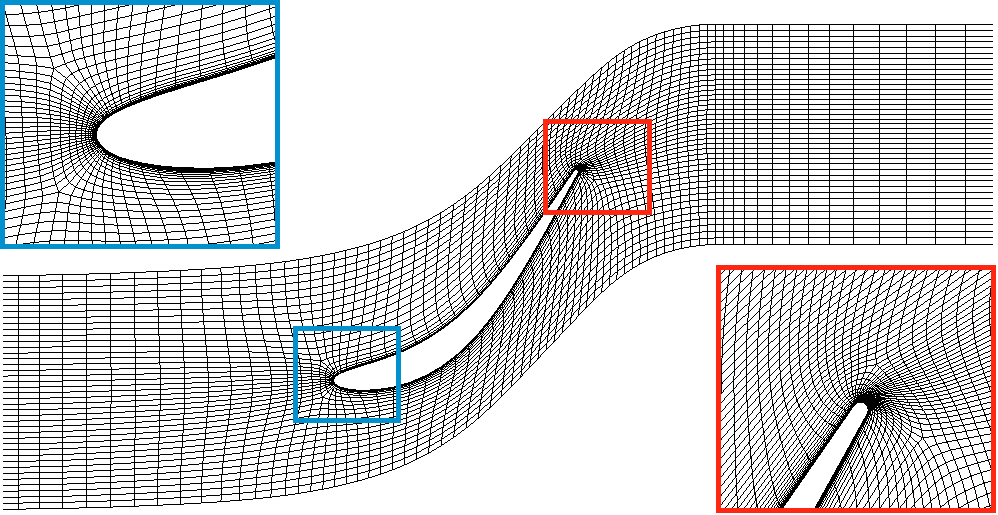
\includegraphics[width=.46\linewidth]{STCF11_MESH.pdf}
  \caption{STCF 11 mesh.}
  \label{fig:stcf11_mesh}
\end{figure}

% boundary conditions
The \textit{elsA}~\cite{Cambier2013} CFD code 
along with its aeroelastic
module~\cite{CIDugeai2011} is used to solve this configuration.
The boundary conditions used for this case are: (i)~an
injection condition  for the inlet (with the relative flow angle,
the Mach number and the total pressure
set to the experimental values using Tab.~\ref{tab:stcf11_steady_results}), 
(ii)~a constant static pressure
condition for the outlet using also the value $p_{s_1}$
given in Tab.~\ref{tab:stcf11_steady_results},  
(iii)~an adiabatic no-slip condition on
blade walls, and (iv)~periodic or phase-lagged conditions 
for azimuthal boundaries depending on the  
prescribed IBPA.

% numerical parameters
Turbulence is modeled using the one-equation model of
\citet{Spalart1992}.  Roe's scheme~\cite{Roe1981} along with a 
third-order MUSCL extrapolation 
is used to compute the convective fluxes.
The classical Dual Time-Stepping~\cite{Jameson1981} (DTS)
time-integration scheme is taken for comparison to the
proposed harmonic balance approach.
The maximum
CFL number is set to~20 for the steady computations,  the inner loop
of the DTS scheme and the HB simulations.  For the DTS scheme,  
convergence in time discretization is obtained
after 20~periods using 128~time steps per period.  Iterative convergence 
for the inner loop is considered achieved when the normalized
residuals drop by $5\e{-2}$ (within a maximum of
50~sub-iterations).

% The steady and unsteady post-processing is done using the
% Antares post-processing software 
% (Appendix~\ref{app:antares}).

\paragraph{Influence of the mesh discretization}
\label{sub:stcf11_mesh_convergence}
The mesh quality is assessed through a mesh convergence.
To ensure the latter, three meshes are tested, the referenced one
described above, and two meshes, coarse~2 and coarse~4,
coarsened in the axial and
azimuthal directions by a factor of two and four, respectively. 
The five grid points in the radial direction
are kept unchanged.

The steady results for the two operating points are shown 
in Figure~\ref{fig:stcf11_mesh_convergence}.
\begin{figure}[htp]
  \centering
  \subfigure[subsonic]{
    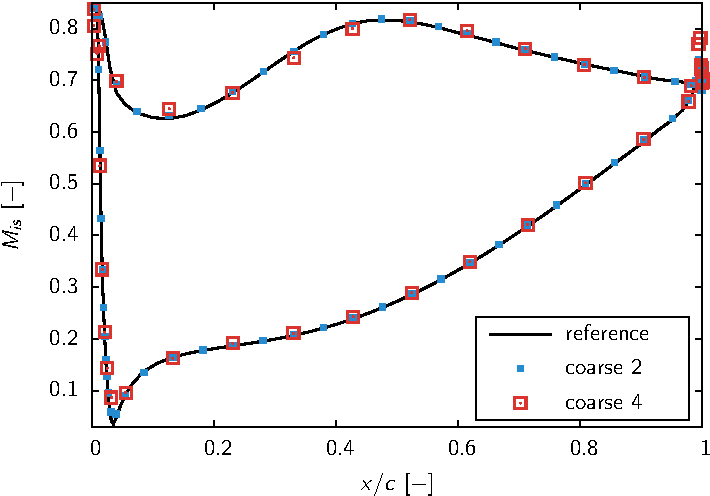
\includegraphics[width=.4\textwidth]{STCF11_RANS_SUBSONIC_CONVERGENCE_MESH_PPT.pdf}}
  \subfigure[transonic]{
    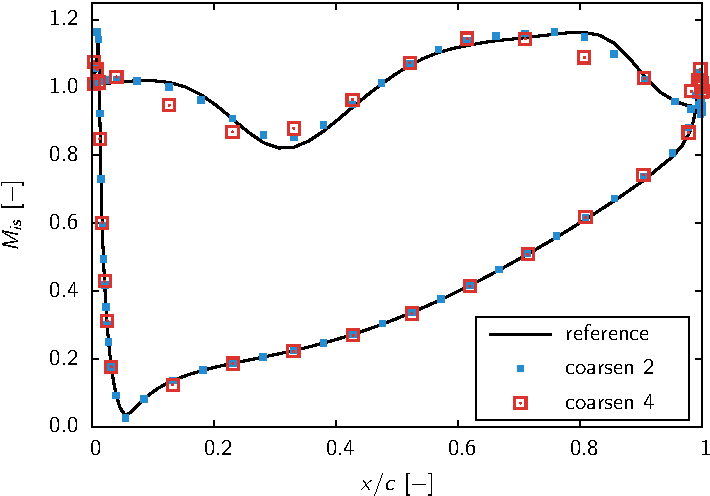
\includegraphics[width=.4\textwidth]{STCF11_RANS_TRANSONIC_CONVERGENCE_MESH_PPT.pdf}}
  \caption{Influence of mesh discretization for the STCF~11 configuration.}
  \label{fig:stcf11_mesh_convergence}
\end{figure}
The three meshes give the same results for the subsonic case. On the
pressure side (bottom curve), the three results are superimposed. On the suction side
(top curve),
some minor differences are observed in particular near the leading edge
($x / c \leq 0.2$). Nevertheless, the agreement
between the three meshes is very good for the subsonic operating point.
The results are more scattered for the transonic operating point. In fact,
the coarse~4 mesh does not accurately predict the region where $x / c \leq 0.3$
and where $0.7 \leq x / c \leq 0.9$. This last zone seems smeared out. 
However, the results
obtained with the coarse~2 mesh are in good agreement with the referenced mesh.
Therefore, the reference mesh is retained for the following study.

\paragraph{Influence of the spatial discretization}
Four space schemes are
used to compute both the subsonic and transonic steady fields. These
schemes are the \citet{Jameson1981} scheme (JST) with artificial
viscosities $\kappa_4 = 0.016$
and $\kappa_2$ equal to $0.5$ and $1.0$ for the subsonic and the transonic
inflow conditions, respectively. In addition to this scheme, three upwind
Roe's scheme~\cite{Roe1981} along with no extrapolation (Roe~1),
a second-order (Roe~2) and a third-order (Roe~3) 
MUSCL extrapolations are used.
The steady results for the two operating points are shown 
in Figure~\ref{fig:stcf11_space_scheme_convergence}.
\begin{figure}[htp]
  \centering
  \subfigure[subsonic]{
    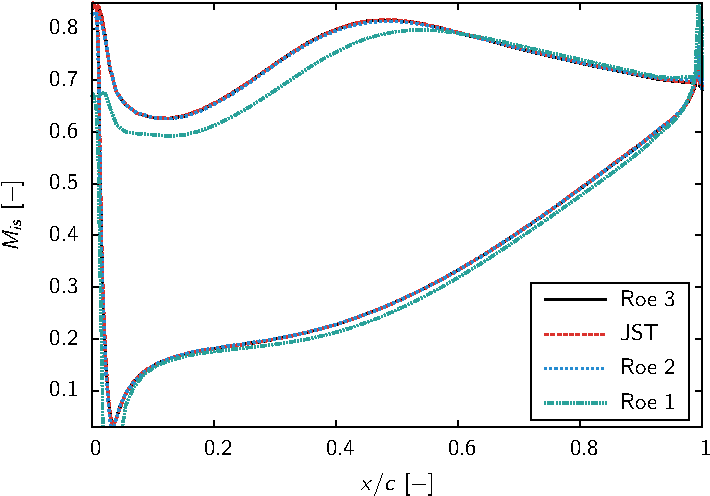
\includegraphics[width=.4\textwidth]{STCF11_RANS_SUBSONIC_SPACE_SCHEME_PPT.pdf}}
  \subfigure[transonic]{
    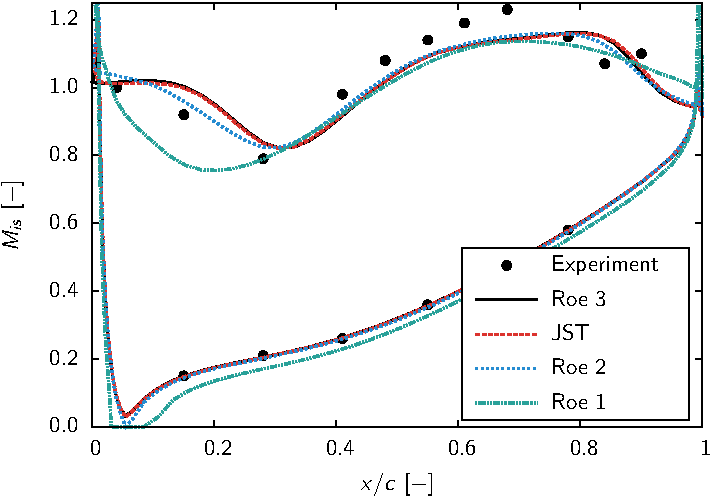
\includegraphics[width=.4\textwidth]{STCF11_RANS_TRANSONIC_SPACE_SCHEME_PPT.pdf}}
  \caption{Influence of mesh discretization for the STCF~11 configuration.}
  \label{fig:stcf11_space_scheme_convergence}
\end{figure}
For the subsonic case, the results are all superimposed except Roe~1. 
This was expected as first-order schemes
are not precise enough to accurately capture turbomachinery flow fields.
For the transonic operating point, which is a numerically stiffer case,
the \citet{Jameson1981} and the Roe~3 scheme are superimposed.
As for coarse meshes, the Roe~2 and Roe~1 schemes
lack in predicting the suction side evolution indicated
by two non-linear flow features: a recirculation
bubble and a shock. In the following,
the Roe~3 scheme is chosen to be the reference spatial scheme.
